\scanpage{244}
\margin{\figure{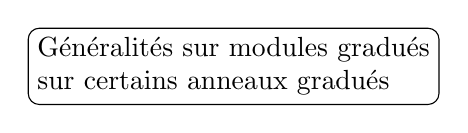
\begin{tikzpicture}\node[draw,rounded corners,align=left] {Généralités sur modules gradués\\sur certains anneaux gradués};\end{tikzpicture}}}
$S$ anneau $\mathbb Z$-gradué \unsure{comm.} à degrés $\geq0$
\[
S^0=k
\]
$\mathcal M$ catégorie des $S$-modules gradués

\figure{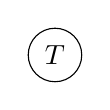
\begin{tikzpicture}\node[draw,circle] {$T$};\end{tikzpicture}} foncteur translation : $T(M)_n=M_{n+1}$
\margin{\figure{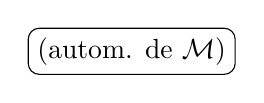
\begin{tikzpicture}\node[draw,rounded corners] {(autom. de $\mathcal M$)};\end{tikzpicture}}}
$T^i$ itéré $i$-ème $(i\in\mathbb Z)$\qquad $T^i(M)_n=M_{n+i}$
\[
\textcircled{$\mathcal M^+$}\subset\mathcal M\quad\big|\quad S\text{-modules gradués à degrés }\geq0
\]
N.B. $\boxed{T^{-1}(\mathcal M^+)\subset\mathcal M_+}$
\[
T^{\unsure{-N}}(\mathcal M^+)=\unsure{\mathcal M_N|\mathcal M_N^*}\qquad S\text{-modules gradués à degrés }\geq N
\]
$(\mathcal M_0=\mathcal M^+)$
\[
N\leq N'\Longrightarrow\mathcal M_N\supset\mathcal M_{N'}
\]
\deleted{$\unsure{\mathcal M}$}
$\mathcal N=$ catégorie des $k$-modules (pas gradués)
\[
M_0\longrightarrow M_0\otimes_kS
\]
\[
\figure{\begin{tikzpicture}\node[draw,ellipse] {$\boxed{\mathcal N\xrightarrow{\varphi}\mathcal M}$};\end{tikzpicture}}\quad\text{se factorise par }\mathcal M^+=\mathcal M_0
\]

\textcircled{1} Étude de l'inclusion (pl. fid.)
\[
\mathcal M_{N'}\underset{i_{N,N'}}{\hookrightarrow}\mathcal M_N\qquad N'\geq N
\]
Commute aux $\varinjlim$ et $\varprojlim$, donc on s'attend à trouver des adjoints à g. et à dr.

\uline{Adjoint à droite} \inserted{$\tau_{N',N}$} \uline{de} $i_{N,N'}$
\[
\tau_{N',N}:\mathcal M_N\longrightarrow\mathcal M_{N'}
\]
\[
\tau_{N',N}(M)_i=\begin{cases}0&\text{si }i<N'\\M_i&\text{si }i\geq N'\end{cases}
\]
C'est un \uline{sous-module} de $M\in\operatorname{Ob}\mathcal M_N$
(car $S$ à degrés $\geq0$)
\margin{\deleted{MATHÉMATIQUES}\par\deleted{PROFESSEUR}\par\deleted{M. GROTHENDIECK ALEXANDRE}\par\deleted{5-856}}
\margin{243}
